\subsection{Energy Storage}
Energy Storage is a large component of Integrated Energy Systems. Currently there are two models of Energy Storage in the repository. Electric Battery Storage, characterized largely as Li-ion battery technology, and two-tank sensible heat thermal energy storage that uses Therminol-66 as the working fluid. 


\subsubsection{Electric Battery Storage}

Electric Battery Storage, shown in Figure \ref{Top View Logical Battery}, is largely characterized as fast and expensive. Due to the speed with which battery storage systems operate, on the order milliseconds, the battery within the hybrid repository has been modeled as a simple logical battery system. The battery can both charge and discharge based upon the direction of electricity flow through the port. It is assumed to be a “perfect” battery and due to the speed of the system, subcomponents have not been modeled simply because they would operate faster than would be useful for the types of analysis utilized with the system. The battery has user-based inputs that control how fast or slow the system can charge and discharge as well as how much energy can be stored within the battery before it is considered full.   

\begin{figure}[hbtp]
\centering
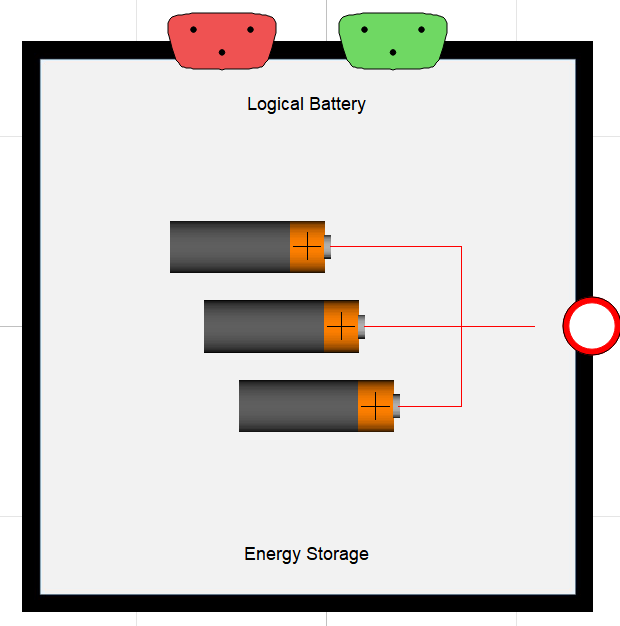
\includegraphics[scale=0.4]{pics/Battery_Storage.png}
\caption{Top Level Depiction of the Logical Battery in the NHES package}
\label{Top View Logical Battery}
\end{figure}


\subsubsection{Two-Tank Thermal Energy Storage}

Sensible heat storage involves the heating of a solid or liquid without phase change and can be deconstructed into two operating modes: charging and discharging. A two-tank TES system, shown in Figure \ref{Top View Two Tank Sensible Storage}, is a common configuration for liquid sensible heat systems. In the charging mode cold fluid is pumped from a cold tank through an Intermediate Heat Exchanger (IHX), heated, and stored in a hot tank while the opposite occurs in the discharge mode. Such systems have been successfully demonstrated in the solar energy field as a load management strategy. The configuration of the TES system held within the repository involves an outer loop interfaces with the energy manifold. Bypass steam is directed through an IHX and ultimately discharged to the main condenser of an Integrated system. An inner loop containing a TES fluid consists of two large storage tanks along with several pumps to transport the TES fluid between the tanks, the IHX and a steam generator. Flow Bypass Valves (FBVs) are included in the discharge lines of both the “hot” and “cold” tanks to prevent deadheading the pumps when the Flow Control Valves (FCVs) are closed. Therminol-66 is chosen as the TES fluid as it is readily available, can be pumped at low temperatures, and offers thermal stability over the range (-3°C–343°C) which covers the anticipated operating range of the light water reactor systems (203°C–260°C). Molten salts (e.g. 48 percent  NaNO3 – 52 percent KNO3) were not considered, as the anticipated operating temperatures fall below their 222°C freezing temperature. The TES system is designed to allow the power plant to run continuously at ~100 percent power over a wide range of operating conditions. During periods of excess capacity, bypass steam is directed to the TES unit through the auxiliary bypass valves where it condenses on the shell side of the IHX. TES fluid is pumped from the cold tank to the hot tank through the tube side of the IHX at a rate sufficient to raise the temperature of the TES fluid to some set point. The TES fluid is then stored in the hot tank at constant temperature. Condensate is collected in a hot well below the IHX and drains back to the main condenser or can be used for some other low pressure application such as chilled water production, desalination or feed-water heating. The system is discharged during periods of peak demand, or when process steam is desired, by pumping the TES fluid from the hot tank through a boiler (steam generator) to the cold tank. This process steam can then be reintroduced into the power conversion cycle for electricity production or directed to some other application through the PCV. A nitrogen cover gas dictates the tank pressures during charging and discharging operation. Full details of the model and its use within integrated energy systems can be found in report \cite{2018ThermalStorage}, \cite{FrickThermalStorage}. 

The model itself is coded in a non-conventional manner compared to the rest of the modelica models. It is coded in an input, output sense rather than in a fluid-port, electric-port based modeling system. This is because the model was transferred over from a FORTRAN style code rather than initially coded in Modelica. To modify the two-tank thermal storage system the user will need to look at each individual model within the charging mode and the discharge mode. Base components within the models are fully commented within the code. Like the HTSE the thermal storage unit is finely tuned and thus use outside of its current state will take a bit of work. To help with this the thermal storage unit has been sized to be compatible for varying sizes of offtake from a power unit. One is sized to take 20 percent of nominal steam from a standard 3400MWt Westinghouse plant, and one is designed for 5 percent offtake. Both designed to provide energy back as a peaking unit. The peaking unit is held within the discharge side of the model and is assumed to have its own turbine or is sent back to the low-pressure turbine. Explicit modeling of the coupling back with the low-pressure turbine has not been done. Future updating of the two-tank thermal storage unit to be consistent with other models is planned.

 
\begin{figure}[hbtp]
\centering
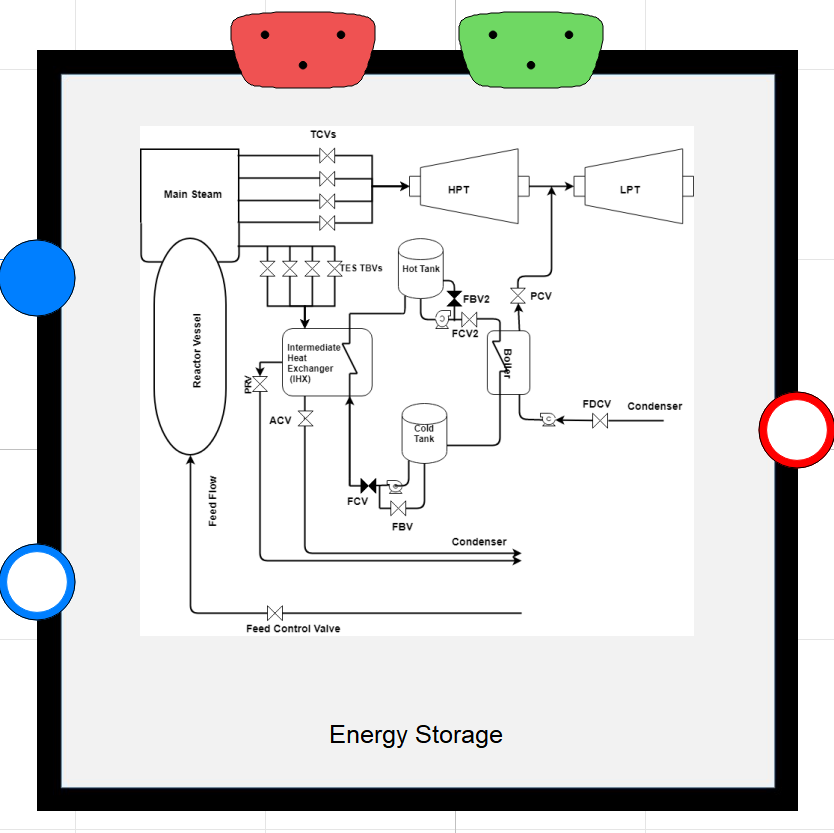
\includegraphics[scale=0.3]{pics/Sensible_Heat_System.png}
\caption{Top Level Depiction of the Two-Tank Sensible Heat Storage Unit in the NHES package}
\label{Top View Two Tank Sensible Storage}
\end{figure}

% content
\subsubsection{Thermocline Packed Bed Thermal Energy Storage}
A thermocline storage system, shown in Figure \ref{Top View Thermocline}, stores heat via hot and cold fluid separated by a thin thermocline region that arises due to density differential between the fluid. Assuming low mixing via internal flow characteristics and structural design, this thermocline region can be kept relatively small in comparison with the size of the tank. Additionally, large buoyancy changes and low internal thermal conductivity are also extremely useful in maintaining small relative thermocline thickness.

To increase the cost-effective nature of these designs, it is common to fill the tank with a low-cost filler material, such as concrete or quartzite. These filler materials are cheap, have high density, and high thermal conductivity. By using such material, a reduction in the amount of high cost thermal fluid can be achieved, thereby increasing the economic competitiveness of such designs.

The thermocline system was modeled from a modified set of Schumann equations that were originally introduced in 1927 \cite{Schumann}. The equation set governs energy conservation of fluid flow through porous media. His equation set has been widely adopted in the analysis of thermocline storage tanks. The modified equations adopted a new version of the convective heat-transfer coefficient to incorporate low and no-flow conditions from Gunn in 1978 \cite{specialHeattransfer}. Additionally, a conductive heat-transfer term was added for the heat conduction through the walls of the tank. Self-degradation of the thermocline in the axial direction is neglected due to low relative values when during standard operation, this is a known limit of the model during times of no flow.

\begin{figure}[hbtp]
\centering
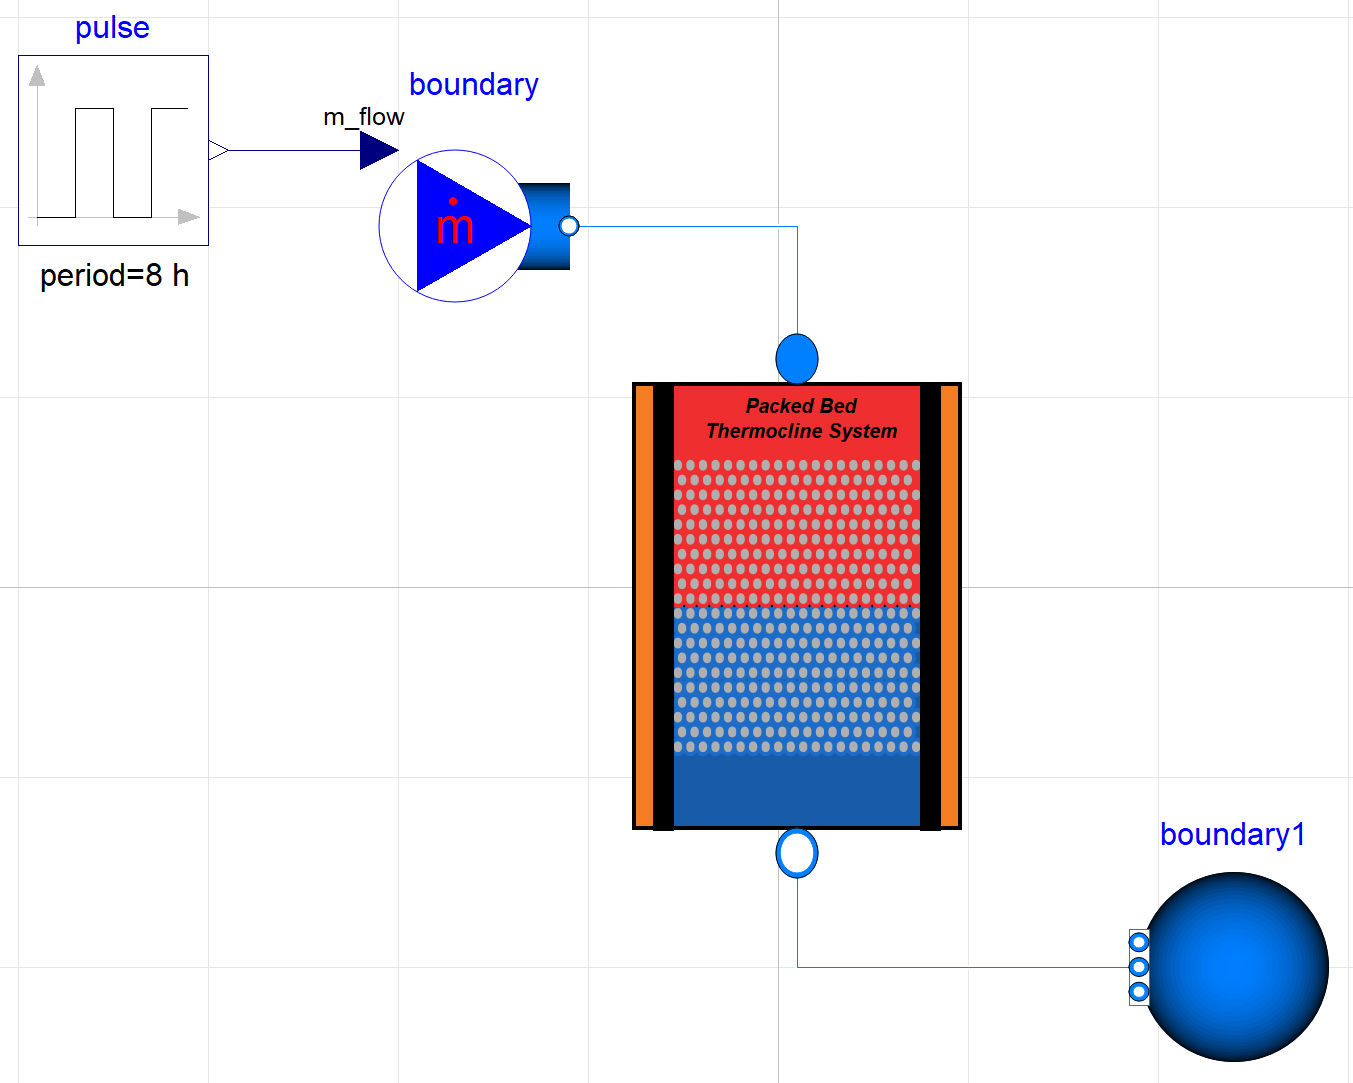
\includegraphics[scale=0.3]{pics/Thermocline_Test.png}
\caption{Top Level Depiction of the Single Tank Packed Bed Heat Storage Unit in the NHES package}
\label{Top View Thermocline}
\end{figure}

\subsubsection{Concrete Solid Media Storage}

Three different models exist for concrete solid media storage, shown in Figure \ref{CTES}. Concrete solid media storage uses inexpensive materials to charge and discharge heat from a fluid system. The models within the Hybrid system use HeatCrete as the concrete material, the properties of which are found in literature. The initial development has been done with energy arbitrage for a Rankine system in mind. However, there are not limitations on the heat transfer fluid that can be used in conjunction with the concrete system. Two design modalities exist with the three developed models. One is a single pipe model and the other is a dual pipe model. All models use simplified flow models: a single pressure and mass flow rate is imposed within a pipe (which allows for significantly improved performance at low and no flow rate conditions) leaving the dynamics of the system to primarily be described by the conservation of energy equation. Within the concrete model, heat conducts both radially and axially in a 2-D nodalized vector. All models calculate values for an average pipe and the system behavior is then scaled by the number of pipes. 

The single pipe model is so called because it only models one fluid pipe within a concrete system. This modeling choice imposes a restriction that heat transfer fluid only flows in one direction or the other (note, no error signals are sent by this, m\textunderscore flow\textunderscore internal = m\textunderscore flow\textunderscore ch-m\textunderscore flow\textunderscore dis). The behavior of this system lends itself better to batch energy applications. The power level during quenching (HTF quenching during charging or concrete quenching during discharging) is an order of magnitude higher than the steady power level. The pressure of the system is taken at the cold end, and defaults to the charging pressure. This model can operate in charging, discharging, OR standby mode. The single pipe model operates with an established axial thermocline and a reversing radial thermal gradient depending on operation. 

The dual pipe and dual pipe two HTFs model contain separate pipes for the charging and discharging flow. This model operates more steadily over long periods of time. Heat is always conducted within the CTES and between the concrete and the HTFs. The dual pipe CTES can operate in charging, discharging, standby, or thermal buffer (both charging and discharging) modes. The dual pipe system operates with mono-directional thermal gradients in both axial and radial directions in all operating modes. 


\begin{figure}[hbtp]
\centering
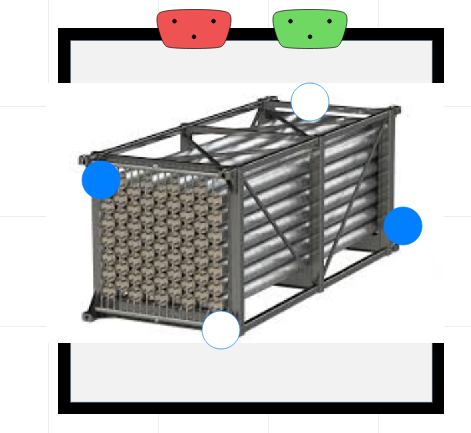
\includegraphics[scale=0.8]{pics/CTES.png}
\caption{Top Level Depiction of Concrete Thermal Energy Storage System}
\label{CTES}
\end{figure}

%\subsection{Cloning the Hybrid Repository}
\label{sec:clone raven}

The first step in installing the package is to clone the HYBRID repository. To do this, use
\begin{lstlisting}[language=bash]
git clone https://github.com/idaholab/HYBRID.git
\end{lstlisting}
This will download the repository into a folder called 'hybrid'. To go inside the folder, use
\begin{lstlisting}[language=bash]
cd hybrid
\end{lstlisting}


\subsubsection{Install RAVEN and its plugins as a sub-module}

The next step is to download and install RAVEN and the submodule (e.g. TEAL, HERON) plugins as a sub-module of the HYBRID repository. 

A submodule allows you to keep another Git repository in a subdirectory of your repository. The other repository has its own history, which does not interfere with the history of the current repository. This can be used to have external dependencies such as third party libraries for example.

In order to get RAVEN do the following in the hybrid folder

\begin{lstlisting}[language=bash]
git checkout devel
\end{lstlisting}

Update the Branch

\begin{lstlisting}[language=bash]
git pull
\end{lstlisting}

to add RAVEN as a submodule
\begin{lstlisting}[language=bash]
git submodule update --init --recursive
\end{lstlisting}

\textbf{Install and Compile RAVEN. }
Once you have downloaded RAVEN as a sub-module, you have to install it. go to the \href{https://github.com/idaholab/raven/wiki/intallationMain}{RAVEN Wiki} for information about how to install it. Run all the tests outlined in the RAVEN wiki. 

\subsubsection{Inform the Framework Paths}

In order to set up the hybrid repository, you must inform the framework about the location of the Dymola python interface. For doing so, navigate to the hybrid directory:

to add RAVEN as a submodule
\begin{lstlisting}[language=bash]
cd <path to your hybrid repository>/hybrid
\end{lstlisting}
Run the following command:
\begin{lstlisting}[language=bash]
./scripts/write_hybridrc.py -p DYMOLA_PATH
\end{lstlisting}

Where DYMOLAPATH is the path to the python interface egg folder in the DYMOLA installation locally. For example:
 
\begin{lstlisting}[language=bash]
./scripts/write_hybridrc.py -p 
	"/c/Program\ Files/Dymola\ 2020x/Modelica/Library/
	python_interface/dymola.egg"
\end{lstlisting}

